\documentclass[12pt]{report}
\linespread{1.5}
\usepackage{mathptmx}
\usepackage[margin=1in]{geometry}
\usepackage{natbib}
\usepackage{graphicx}
\usepackage{setspace}
\usepackage{textcomp}
\usepackage{graphicx}
\usepackage{subcaption}
\usepackage{listings}

\begin{document}


\begin{titlepage}
\begin{center}
B.Comp. Dissertation\\
\vspace{3cm}

{\large\textbf{Tools for Security Senario Setup}}

\vspace{5cm}

By\\

Sun Mingyang

\vfill
% 
\includegraphics[width=0.4\textwidth]{./pictures/nus-logo}

Department of Computer Science\\
School of Computing\\
National University of Singapore\\
2018/2019
\end{center}
\end{titlepage}


\begin{titlepage}
\begin{center}

B.Comp. Dissertation
\vspace{1cm}

{\large\textbf{Tools for Security Senario Setup}}

% Orchestration Tool for IT Network Traffic Generation\\
% and Human Behavior Simulation in Web Browsing

\vspace{4cm}

By\\
Sun Mingyang\\
\vspace{2cm}
Department of Computer Science\\
\vspace{0.3cm}
School of Computing\\
\vspace{0.3cm}
National University of Singapore\\
\vspace{0.3cm}
2018/2019\\
\end{center}
	
\vfill

\begin{flushleft}
Project ID: H0041300\\
Project Supervisor: Assoc Prof Change Ee-chien\\
\vspace{0.5cm}
Deliverables:\\
\setlength{\parindent}{30pt}
Report: 1 Volume\\
Manual: 2 Volumes\\
Program: 1 Git Repository\\
\end{flushleft}
\end{titlepage}


\begin{abstract}

Normally, during Cyber Defence Exercise (CDX), it would be relatively easy to perform an attack or deploy an exploit once the vulnerability is known, however, setting up an appropriate security senario or target system  will be rather difficult.
In a particular example, during a Cyber Defence Exercise targeting a virtual enterprise-scale network, the attacking traffic performed by the Red Team (who will conduct the attacks) may be too obvious to be spotted or identified by the Blue Team (who will defense the network) when the attacks are performed in the an ``empty" virtual network where there is no background noise or ``normal" web traffic. \\

The goal of this project is to build tools that could help to simulate the real-world scenario and generate normal and benign network traffics in the virtual environment during the CDX similar to what has been described above.\\

This project will consist of two compoents, while the first one is to build an orchestration tool for generating a sufficiently large amount of network traffic in a distributed system senario, and the second one is to simulate human behaviors in web browsing to make the web traffic more realistic.\\

The evaluation and demonstration of this project will be conducted in the virtual network  provided by the National Cyber-Security R\&D Lab (NCL) and the final product may have international impacts on the CDX held by KYPO Cyber Range in Czech Republic.\\

\pagebreak

\setlength{\parindent}{0pt}
\textbf{Subject Descriptor:}\\
C.2.4: Distributed Systems\\
D.2.2: Design Tools and Techniques\\
D.2.3: Coding Tools and Techniques\\
D.2.13: Reusable Software\\
G.3: Probability and Statistics\\

\textbf{Keywords:}\\
Cyber Defence Exercise Setup, Orchestraction Framework, IT Network Traffic Generation, Network Security, Distributed System, Human Behavior Simulation\\

\textbf{Implementation Software:}\\
Ubuntu Linux 18.04 Bionic Beaver, Python 3.6, Flask 1.0, Flask-Marshmallow 0.10, Flask-SQLAlchemy 2.3, Marshmallow-SQLAlchemy 0.16, Selenium 3.141, SQLAlchemy 1.3, osBrain 0.6, APScheduler 3.5, ntlk 3.4, React 16.6+, Ant Design 3.10+\\

\end{abstract}

\chapter*{Acknowledgements}
\thispagestyle{empty}
\begin{spacing}{2}
\setlength{\parindent}{0pt} I wish to express my sincere thanks to Chang Ee-Chien, Associate Professor from School of
Computing, National University of Singapore, for providing me with all the necessary information and facilities for this project.\\

\setlength{\parindent}{0pt} I place on record, my sincere thank you to Dr. Jan Vykopal from National Cyber-Security R\&D Lab (NCL), for the continuous help. I am extremely thankful and indebted to him for sharing expertise, and sincere and valuable guidance and encouragement extended to me.\\

\setlength{\parindent}{0pt} I am also grateful to Ivo Nutar from the Institute of Computer Science, Masaryk University, Brno, Czech Republic, for sharing with me lots of relevant work and past experience while I am developing the project.\\

\setlength{\parindent}{0pt} Finally, I will also take this opportunity to express gratitude to all of the members in NCL who everlent their hands to me along this project for their help and support.\\
\end{spacing}
\clearpage

\tableofcontents

\chapter{Introduction}
\section{Background}
Practical Cyber Defence Exercise (CDX) creates virtual network environment and helps participants experience and understand how attacks against the infrastructures in their organizations are performed. The Blue Team (i.e. defenders) in CDX are normally supposed to come up with countermeasures and deploy some defending actions against a large variety of attacks that will be performed by the Red Team (i.e. attackers), as well as to monitor the context or the environment, a virtual network in most of the case, for any suspicious traffics or actions, or to recover from some successful exploits.\\

Since the CDX should simulate the real operational network environment as much as possible, instead of attacking traffics, there should be plenty of benign and normal web traffic existing during the CDX as well. In such case, the quality and accuracy of benign traffic has a significant impact on the learning experience and the effectiveness of the whole security exercise because usally we do not want the attacks to be the only traffics in the virtual network. Therefore, ensuring that the quality and volume of background traffic is able to camouflage the attacking traffics from any automated intrusion detection systems will be an very essential goal to set up the CDX virtual environment, or otherwise, it will be too trivial for the Blue Team to detect intrusive traffics.\\

To achieve the goal above, a large amount of background traffic that simulates actions performed by normal users or actual humans should be guaranteed. Many current practice of simulation of normal traffics in CDX may engage human beings or hard-coded traffic generators, for example, to use dedicated scripts or softwares on every individual machine, which are neither scalable nor efficient, especially when there is a dramatic system requirement change. Besides, as the scales of many CDX are enlarging quickly, more operators or clients will be needed to produce enough realistic network traffic. As a result, automating the process of generating sufficient amount of high-quality benign traffic according to a reasonable amount of configurations is becoming neccessary. And this is also the main goal of this project.\\

To fulfill the requirements illustrated above, we are going to propose a brand-new framework to simulate abd generate normal traffic during CDX, based on some state-of-the art works on automotive traffic generating and some studies on real human behavior. This framework will involve multiple client nodes and a controller node. Each of the clients will play a role of a fictitious user to simulate a normal network user who is performing regular actions such as web browsing and sending emails, while the controller node will play a role of an orchestrator, who is going to instruct all the clients based on some configurations, as well as to monitor system status on each client machine.\\

As for the types of traffic that will be generated by this framework, we will primarily focus on email and web traffic in this project. This is because these two kinds are of the most common activities that the internet users will have, while the portion of web traffic in the whole internet traffic mix has became dominant \citep{IATMA}. But we will also open the options and possibilities by design and implementing a highly extensible framework for the future for more types of traffic. Furthermore, since there is a much larger degree of randomness in web browsing behaviors of humans, we will also design and implement an algorithm or a mathematical model to predict or reproduce the realistic human web browsing traffic.\\

In this report, chapter \ref{rw:tfo} and chapter \ref{sd} will mainly focus on the scope of the design of orchestration tool, while chapter \ref{lr:hwbs} and chapter \ref{mm} will mainly talk the methods that will be used to simulate human behaviors. Last but not least, chapter \ref{imp} will address on the actual implementation.

\section{Illustration of actions to be done by fictitious users in CDX} \label{senario}

Based on the background we illustrated before, here, we are going to elaborate a more specific scenario where a ``fictitious" user or a client is created and what it is supposed to do in order to generate “normal traffic” during a CDX. The fictitious users will reside in a virtual network created during CDX, and there will be numerous of them existing simultaneously to ensure the traffic volume. The actions specified below describes the actions needed to be performed by a certain client during CDX, and these actions will be executed on a routine base (i.e. repeat every day or every few hours) and will stop until the CDX ends.\\

\setlength{\parindent}{0pt}
\begin{tabular}{ | c | c | c | c | c |}
\hline
\multicolumn{3}{|c|}{Client LAN IP: 10.0.26.4}&\multicolumn{2}{|c|}{Browser: Chrome}\\
\hline
\hline
\textbf{Time} & \textbf{Actions} & \textbf{Data} & \textbf{Destination} & \textbf{CDX actions}\\
& & & \textbf{application/service} & \\
\hline
8:00 to 9:00 & Browsing & N/A & www.bbc.com & Red Team will\\
& news sites & & www.cnn.com & disable DNS in \\
& & & & the virtual network.\\
\hline
9:00 to 10:00 & Send emails & email account & admin1@ncl.org & Red Team performs\\
& to a list of & credentials & admin2@ncl.org & MITM attack and \\
& email address & & & hijack the email traffic\\
\hline
10:00 to 11:00 & Check whether & email account & www.nclweb1.org & Some web services\\
& some internal & credentials  & www.nclweb2.org & in Blue Team virtual \\
& web services & & & network will be \\
& is accessible & & & under DoS attack\\
& (if not, send & & & by Red Team.\\
& email to admin) & & & \\
\hline
11:00 to 11:30 & Check external & N/A & www.google.com & The website will\\
& websites & & & be defaced by\\
& & & & the Red Team. \\
\hline
\end{tabular}\\

\section{The need of an automatic traffic generator to simulate human behaviours in CDX} \label{assumption}
% TODO to be refined.
Since most of the actions specified in the previous section are referenced from the actual actions to be done during some CDX held by NCL, and are actually achieved by actual humans. These tasks are nearly impossible to be directly repaced by automation scripts or softwares since they introduce lots of randomness and decision making in terms of human behaviors. However, this method will become really expensive when the scale of CDX becomes larger. Thus, we would like to propose a traffic simulator which could not only orchestrate a large scale distributed system, but also be able to include modules that could simulate human behaviors.\\

In the context of the table above, our proposed framework will help to schedule and execute all the entries appeared in the ``Actions" coloumns, where the users of our framework (e.g. CDX cordinators) will only need to provide the information appeared in ``Time", ``Data" and ``Destination" coloumns.

\section{System design requirements}

In this part, we would like to define all major requirements that our proposed traffic generating orchestration framework and the spsecific math model for human behavior simulation should satisfy. In the context of this project, the software or framework delivered will be the taffic generating orchestration tool, while the human web-browsing behavior simulation model will be one of the key modules in the framework, which would only help to generate web browsing traffics.

\subsection{Requirements for Traffic Generating Orchestration Tool}
\label{framework-requirements}
\begin{enumerate}
\item \textbf{Modular architecture}: Modular software architecture should be achieved to enable extensibility and efficient development of individual components in parallel.
\item \textbf{Distributed system with controller}: There should be a controller acting as an orchestrator to instruct a number of clients that acts as ficticious users distributed at various hosts in virtual environment, and the controller and the clients should be able to communicate seamlessly.
\item \textbf{Real clients and tools are used}: Real clients and tools are used for generating realistic traffic. In other words, forged traffic or crafted packets should not be injected to network, but interactive sessions between clients and web services are established.
\item \textbf{Extensibility of protocols is supported}: Framework can be extended to generate traffic of various network and application protocols. For this project, we will only involve protocols that are related to web browsing (e.g. HTTP/HTTPS) and email (e.g. POP3/IMAP) first. But we will also ensure the high extensibility for the framework.
\item \textbf{Client-side cross-platform supported}: Client side framework should be deployable at least at Linux and Windows operating systems.
\item \textbf{High-level script of actions supported}: Traffic will be generated according to a human-readable high-level script of actions (which will be explained in more details in a later section) provided to the controller node by an human operator beforehand. The operator is able to specify fictitious users with their routine or scheduled actions, but not network packets nor flows. For example, valid actions may refer to ``browsing the news website", ``sending an email to X", or ``check web service Y, if not accessible, send email to admin, and if accessible, go to ther service and upload file Z".
\item \textbf{Scheduled/repeatable/conditional actions}: Actions defined in the high-level script should be able to be executed either according to a scheduled timeline (repeatable/non-repeatable) or certain conditions specified by the operator.
\item \textbf{On-demand actions}: Traffic can be also generated on-demand during the execution of the scheduled script. Framework provides a simple way for the operator how to instruct all clients from the controller.
\item \textbf{Graphical user interface}: The framework should provided a graphical user interface for the controller, enabling the operator to instruct and monitor the clients’ status and traffic status in real time with minimum effort.
\item \textbf{Dynamic plan for taffic generation}: The framework should give some flexibility for the operators to dynamically change the traffic generation plans in the middle of generation stage.
\end{enumerate}

\subsection{Requirements for Human Web-browsing Behavior Simulation Model}
\begin{enumerate}
\item \textbf{Continuous generation of traffic}: The model designed should be able to continously generate web traffic without any interruptions unless specified or instructed. 
\item \textbf{Simulation of human behavior}: The model should be able to simulate how a real human being browses web pages to a certain degree. For example, if we want one ficticious user to browse inside a news website, it will be more likely for him to navigate through many news pages, but rather less likely to end up in clicking an advertisement link after a few minutes.

\end{enumerate}

\chapter{Related Work: Traffic Generating Orchestration Tool} \label{rw:tfo}
In this chapter, we would like to review a few relevant projects about traffic generation tools and framework as well as some of their key features, which we could potentially benefit from.

\section{BrowSim}

BrowSim \citep{BrowSim} is a web traffic simulator developed in Python. It makes use of Selenium framework for web traffic generation and Vagrant to manage all virtual machines (i.e. clients) involved. It supports both local web traffic generation where the traffics are merely produced by the machine where BrowSim is installed, and distributed web traffic generation where there is a hub (as a controller) to monitor and control all other nodes (as clients).

\subsection{Usage}

To use this tool, the user will utilize the provided API (which are just defined by python functions, and are also known as ``browsing functions" in BrowSim\textquotesingle s defination) to write a python script for each of the client nodes to explicitly specify their behaviors.\\

Essentially, BrowSim provides four browsing functions/APIs for web traffic generation:

\begin{itemize}
\item \textbf{keyword searching}: The user will apply this function to let the node search for certain keywords using a common searching engines as specified. The searching engine can be specified by passing a sting parameter when this function is called.

\item \textbf{news site crawling}: The user will apply this function to let the node crawl through a certain news website as specified in one of its parameter. The user will also need to specify how the crawling will happen -- by ‘clicking’ the ``visually largest" hyperlink, or one of the first ten ``visually largest" hyperlink, or just a random hyperlink inside the current webpage every time the Selenium web driver decides to proceed to a new webpage.

\item \textbf{website logging in}: This function will try to login to a webpage, such as a social media website, according to user-specified username and password (provided as function parameters).

\item \textbf{execute a file}: This function will execute a given file (where the file path in provided by a function parameter) using the Selenium webdriver.

\end{itemize}

\subsection{Discussion}

BrowSim is good enough to automatically generate a large amount of web browsing traffic, provided with some level of user customization. It can also be easily extended by implementing more powerful browsing functions with more robust browsing logic or predictions. And the Selenium framework it used is a really powerful tool for developers to conduct network reliability test or traffic simulation related to web browsing.\\

However, as all behaviors and logic flows happening on each node during generation are spcified by the user crafted python script, the customization for different nodes becomes very expensive, and an operator who is lack of python programming skills may not be able to adept it very quickly. Besides, the communication between each clients and the controller will happen every time when there is a new traffic to be generated, which injects lots of unnecessary traffics to the network. Another major problem is that BrowSim is not scheduler-based, which means creating iterative actions or scheduled actions will become expensive or even impossible during CDX.

\section{Yoshka}

Yoshka \citep{Yoshka} is a platform-independent framework that aims to generate high-fidelity network traffic and create lifelike virtual environment during CDX. The traffic is scheduled and generated based on a behavior tree compiled from a user specified high-level script written in YMAL, a human-readable serialization language widely used in configuration files.\\

Behavior tree \citep{BT1} \citep{BT2} is basically a directed acyclic graph commonly used in game development industry to determine the behaviors of non-playable characters (NPC). To further simplify the behavior logic, Yoshka makes use of binary trees which will restrict the outcome of each vertex in behavior tree to only “success” and “failure”. Below are examples of the high-level script of actions and the behavior tree used in Yoshka.\\


\begin{figure}[h!]
  \centering
  \begin{subfigure}[b]{0.45\linewidth}
  	\centering
	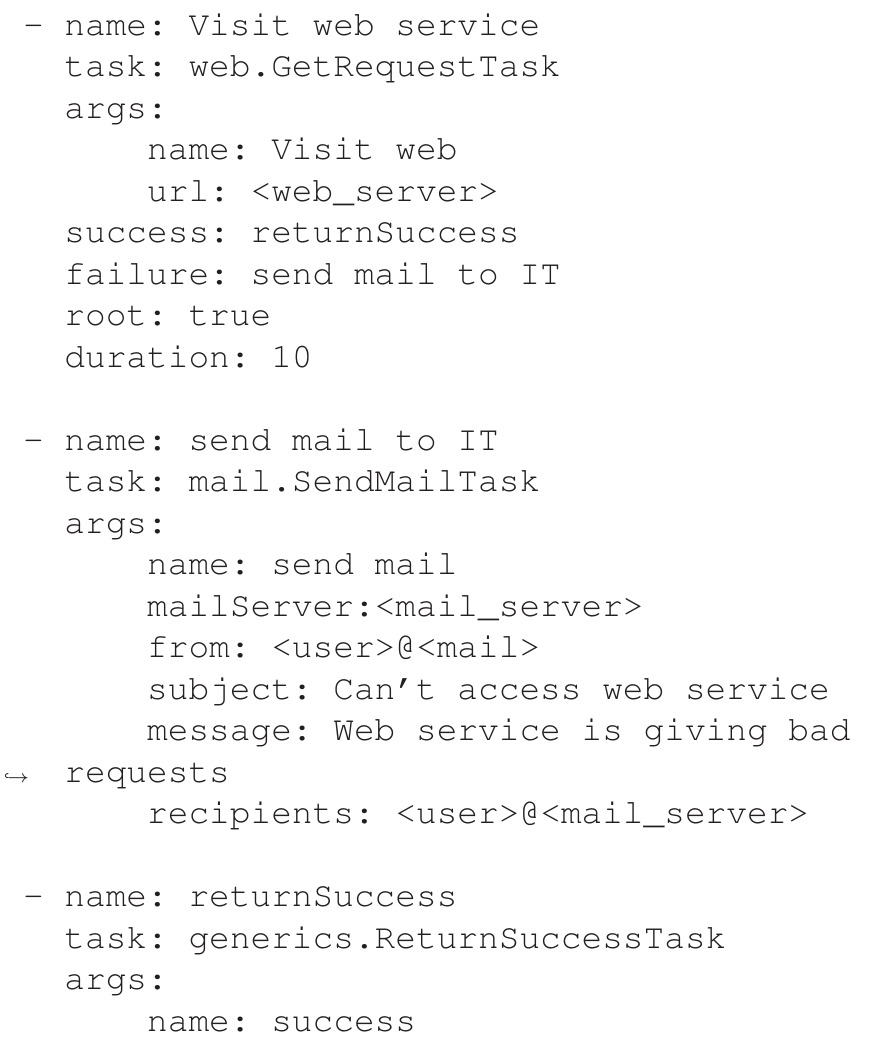
\includegraphics[width=1\textwidth]{./pictures/yoshka-hls}
    \caption{High-level Script}
  \end{subfigure}
  \begin{subfigure}[b]{0.45\linewidth}
	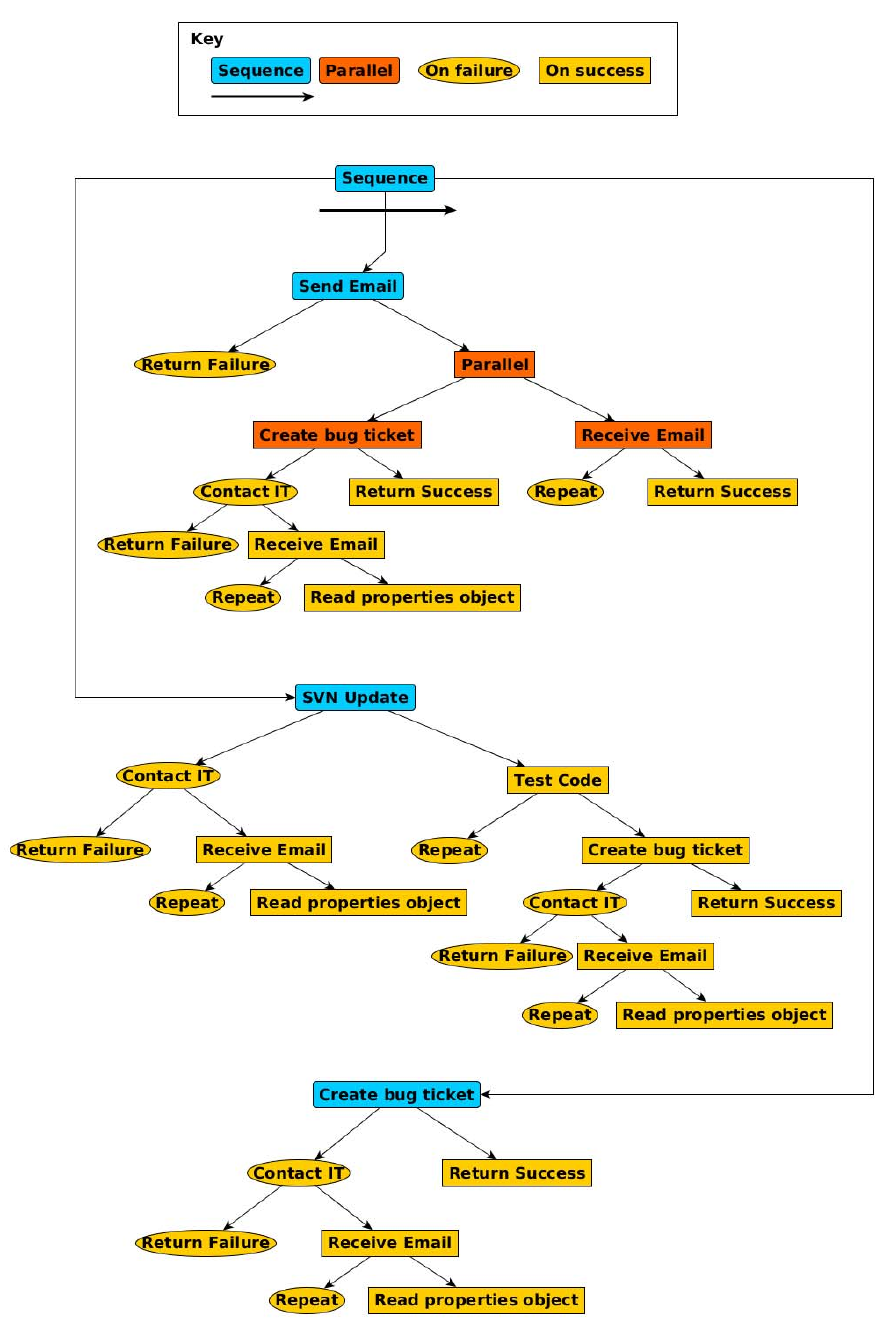
\includegraphics[width=0.9\textwidth]{./pictures/yoshka-bbt}
    \caption{Binary Behavior Tree}
  \end{subfigure}
  \caption{Examples and Concept Illustration in Yoshka}
\end{figure}

\subsection{Discussion}

Yoshka provides support for a wide spectrum of network traffic, such as mail traffic, ftp traffic and web browsing traffic, along with a graphic interface on controller node to monitor the real-time status of network traffics and other client machines. Moreover, Yoshka is also of a very high extensibility for new type of traffic or protocols to be added on, which provides a lot more adaptability to changing scenarios and conditions in CDX.\\

Nevertheless, because Yoshka is a closed project, people outside their institute will not be able to access the source codes. But we can always brought some valuable concepts from this project through what they have already published, such as the idea of how to make use of binary behavior tree to construct the human readable high-level script. 


\section{Cryton}

Cryton is an extensible framework written in Python developed by \citet{Cryton} from the Institute of Computer Science, Masaryk University, Brno, Czech Republic, and was originally designed to automate the attacking process (or generating attacking traffic) during CDX. This framework was developed based on client-server architecture, where a centralized sever/controller will orchestate all client behaviors. It implemented a similar idea of binary behavior tree in Yoshka, and it also makes use of high-level script of actions (written either in JSON or YMAL) for user specification.\\

Cryton introduced a concept called ``modules", each of which represents a specific ``attacking" action and will only be deployed on the client machines. There are plenty of pre-prepared modules could be used in Cryton, such as ``mod\_scanner" module which will make use of the nmap tool to scan a certain IP address on certain ports, and ``mod\_msf" module which will make use of certain metasploit resource to conduct corresponding exploits or attacks. An example of the high-level script of actions is shown in the figure below:

\begin{figure}[h!]
	\centering
	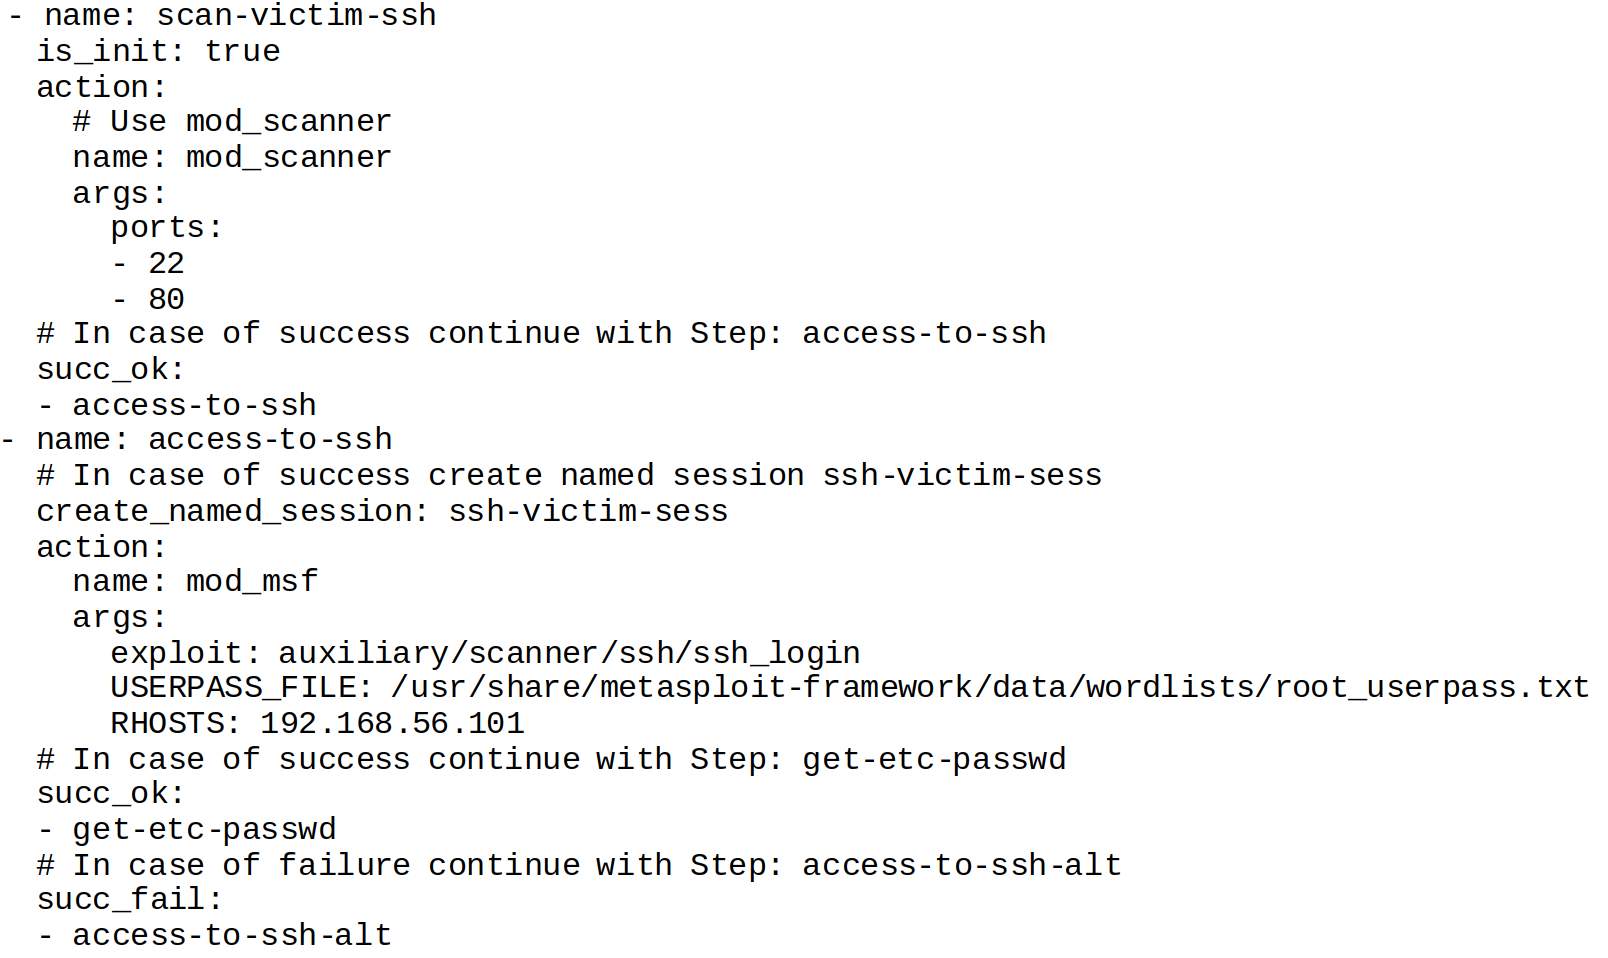
\includegraphics[width=0.8\textwidth]{./pictures/cryton-hls}
	\caption{Example of high-level script used in Cryton}
\end{figure}

\subsection{Design Architecture}

Thanks for the support from the author, \citet{Cryton}, we could get the chance to access the original source code and examine and learn from the software architecture of Cryton. The figure below is a high-level review of how Cryton was implementing the server-client software architecture, and here in Cryton implementation, word ``master" is used to define the controller/server node, while word ``slave" is used to for client node.

\begin{figure}[h!]
	\centering
	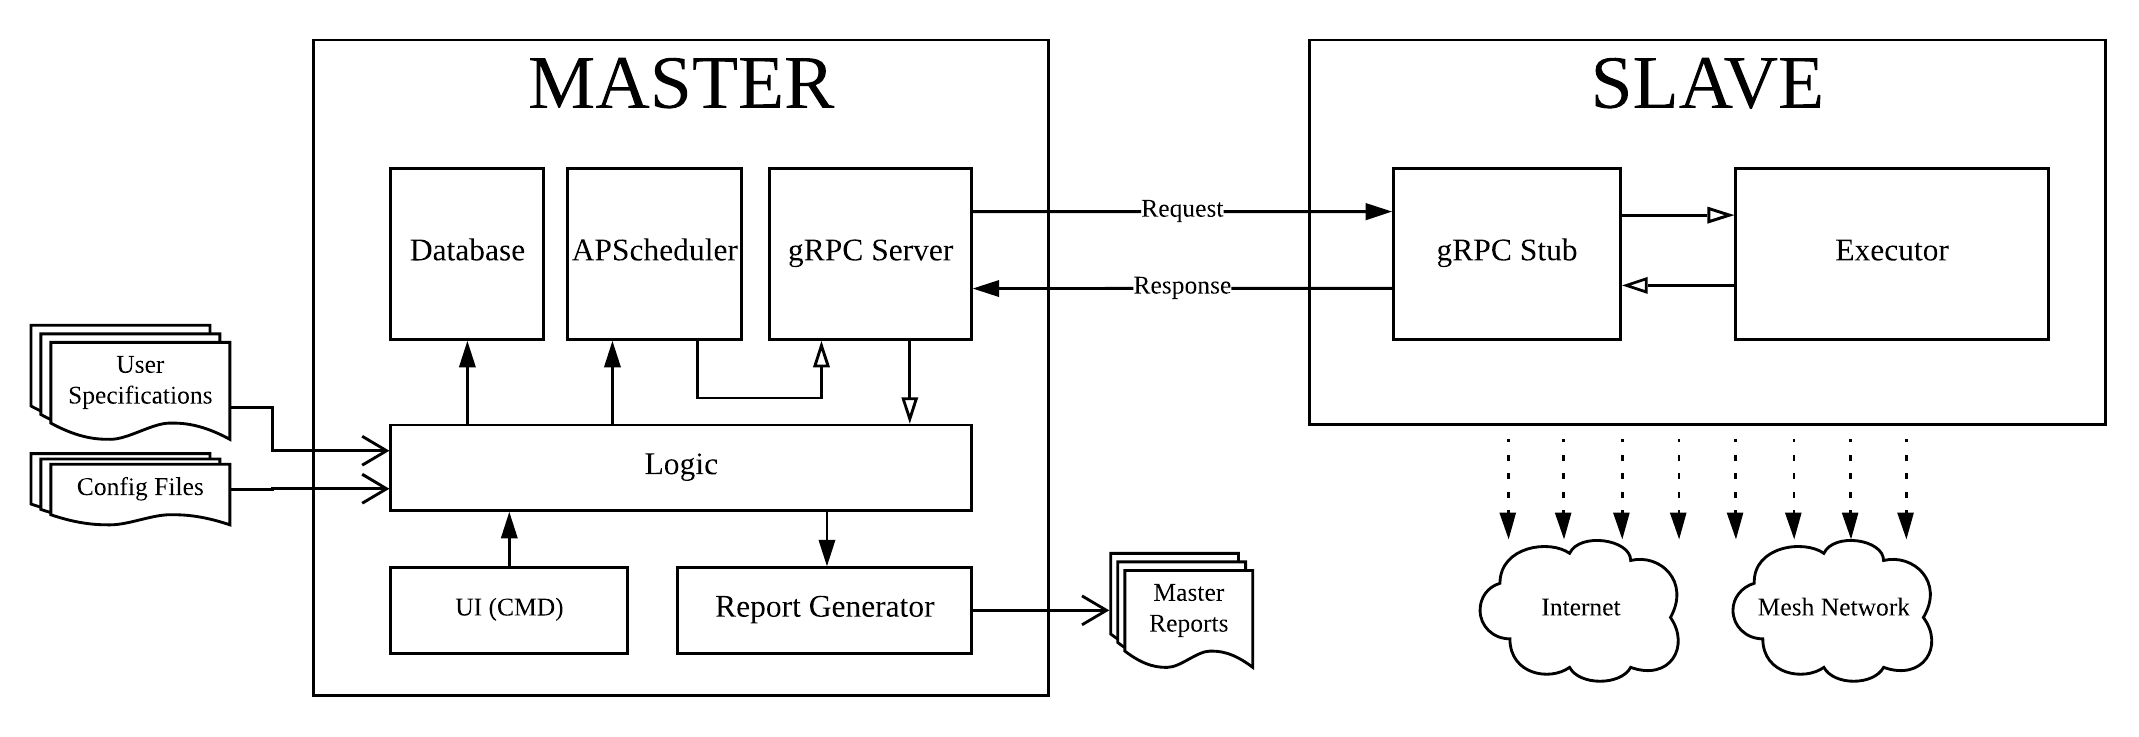
\includegraphics[width=1\textwidth]{./pictures/cryton-arc}
	\caption{Software architecture of Cryton}
\end{figure}

Basically, the user of Cryton will interact with Cryton through a command-line user interface on the master node. He or she can pass in a high-level script of actions that specifies the slave behaviors slaves. Then it will become master\textquotesingle s responsibility to parse the input file, generate the behavior tree logic and then schedule the tasks or actions accordingly. When certain tasks are to be executed, the master will notify and give the instruction to the slaves and the slaves will execute the “modules” and return the execution status (“success” or “failure”) back to the master to generate an execution report.


\subsection{Discussion}
While there are quite a few design concepts we could learn from Cryton, there are also several major limitations about Cryton explaining why we may not be able to extend it to fulfill our project requirements. Here, we are going to discuss three major ones.\\

First of all, in attacking scenario, consecutive actions are connected or linked via “session” (e.g. ssh session or tcp session) and the decision of action flow may merely depend on a binary status (i.e. either success or failure), for example, once an SSH session is created successfully, Cryton may remember the name of the session and return a “success” code for the next action to start execution based on the existing session. However, for the actions or tasks to be used for normal web traffic generation, the behaviors may highly depend on the real output (e.g. an HTML page) from its predeceasing action, which cannot be simple achieved by the binary behavior tree implemented in Cryton.\\

Secondly, in Cryton, every action can only be scheduled for once. The scheduler implemented on master node does not support any iterative tasks. Though repeating tasks can still be created by passing in multiple identical high-level script of actions at different time stamp, this process may become very trivial and this will become much less intuitive for the users.\\

Thirdly, every action is scheduled on master node, presenting a lot of overhead on the controller machine as well as some delay of execution for some tasks. Though multiple threads will be created for each individual chain of actions, the overhead and the delay will still be inevitable as the number of slave nodes increases. For example, if there are one hundred tasks scheduled on one hundred slaves at a certain time point, the master node must instruct these one hundred slaves simultaneously to finish all task execution. 

\section{DumpsterFire Toolset}
The DumpsterFire toolset \citep{Dumpsterfire} is an open source project for creating scheduled, repeatable and distributed security events during CDX. By saying security event, it may refer to any actions done by either Red Team or Blue Team during CDX. Each atomic action is called DumpsterFire, and the user can schedule the DumpsterFire as they need.\\

DumpsterFire toolset is modular, cmd-menu-driven, cross-platform and easily extensible. However, the major issue with DumpsterFire toolset is that this tool may not be able to deployed on a distributed senario. It will be really helpful for a specific memeber in either Red Team or Blue Team to use this tool to save their time on some trivial or standardized actions. However, to meet the requirements of the CDX we specified before, each client machine needs to be installed with a DumpsterFire toolset and configured seperated. Besides, to schedule a DumpsterFire, there is no easy way such as passing in an input configuration file, but the user have to use the command line interface to specify and configure each task explicitly.

\section{AutoTTP}
AutoTTP (Automated Tactics Techniques \& Procedures) \citep{AutoTTP} is another open source project that aims to simplify only the attacking procedures during CDX. Again, it is not capable to generate a sufficient amount of traffic since this tool does not support distributed deployment and it is hard to be extended to generate normal traffic since most of its atomic actions are dependent on some attacking frameworks.\\

\section{Summary}
As we have explored a few existing tools or frameworks for traffic generation (either for normal traffic or attacking traffic), no one of them are very suitable to be applied or extended to our scenario, though some of the design decisions and concepts can be learnt and studied. Here is a table of summary on how these related projects fit our project requirements specified in section \ref{framework-requirements}.\\

\setlength{\parindent}{20pt}
\begin{tabular}{ | c | c | c | c | c | c |}
\hline
                     & BrowSim & Yoshka & Cryton & DF toolset & AutoTTP\\
\hline
Modular architecture & NO & YES & YES & NO & NO \\
\hline
Distributed system & YES & YES & YES & NO & NO \\
\hline
Real clients and tools & YES & YES & YES & NO & YES \\
\hline
Extensibility of protocols & NO & YES & YES & YES & YES \\
\hline
Client-side cross-platform & YES & YES & YES & - & - \\
\hline
High-level script of actions & NO & YES & YES & NO & NO \\
\hline
Scheduled actions & NO & YES & YES & YES & YES \\
\hline
Repeatable actions & NO & YES & NO & YES & YES \\
\hline
Conditional actions & NO & YES & YES & NO & NO \\
\hline
On-demand actions & NO & YES & YES & YES & YES \\
\hline
Graphical user interface & NO & YES & NO & NO & NO \\
\hline
Dynamic scheduling plan & NO & - & NO & NO & NO \\
\hline
Access to Source & YES & NO & YES & YES & YES \\
\hline

\end{tabular}


\chapter{System Design: Traffic Generating Orchestration Tool - Autraff} \label{sd}

In this section we are going to propose our own framework, Autraff, for traffic generation to satisfy the requirements specified in section \ref{framework-requirements}. Firstly we will introduce the software architecture followed by detail explanation of each single component. Then we will show an example work flow from the user perspective and inroduce the high-level script used by users in our framework. Last but not least, some implementation details will be illustrated in the last section.

\section{Terminologies}
Before we start, we would like to first clarify some terminologies used in our system.\\

\setlength{\parindent}{0pt}
\begin{tabular}{ | l | l |}
\hline
\textbf{Term} & \textbf{Meaning} \\
\hline
Cient & Referring to the actual node in the network that is used to generate the network \\ & traffics. \\
\hline
Controller & Referring to node where the orchestrator (which is used to manage all client nodes) \\ &  of the orchestration framework is installed. \\
\hline
UI & In the content of Autraff, most of the time UI refers to a graphical user interface. \\
\hline

\end{tabular}

\setlength{\parindent}{0pt}
\begin{tabular}{ | l | l |}
\hline
\textbf{Term} & \textbf{Meaning} \\
\hline
Module & It is used to define a type of atomic actions that will be stored on the client side. For \\ 
& example, module ``mod\textunderscore visit\textunderscore any\textunderscore page" defines a type of actions that will visit one \\ 
& specific web page only. \\
\hline
Argument & Each module will consist of several arguments which will decide the exact behaviors \\ & of a module. For example,  module ``mod\textunderscore visit\textunderscore any\textunderscore page" may have an argument \\ & called `url' to tell the module to visit which web page and another argument called \\ & `time' to tell how long this module should stay on this page before leaving/closing.\\
\hline
Job & It is a definition to represent the actual actions that will be performed by the client. \\
& Each job will make used of exactly one module, and it will also define when the  \\
& action will be excuted and consist of all arguments needed to execute a module. Two \\ & different job can use the same module but with different arguments.\\
\hline
Start Time & Some jobs may be defined with a start time which denote the time when this job is \\ & executed for the first time. \\
\hline
Interval & Some jobs may be defined with an interval attribute, which denote the time interval \\ & between the two consecutive execution of the same job. \\
\hline
Schedule & When used as a verb, this word means to schedule a job on a specific client according \\ & to how this job is defined. Note that, not all jobs can be schedule since some \\ & jobs may be triggered by some events.\\
\hline
\end{tabular}

\section{Software Architecutre and Overview}

In this section we are going to present the high-level architecture design of Autraff. Basically, it follows the server-client architecture inspired by Cryton \citep{Cryton}, but we have designed it to make it more suitable to fit our assumptions and senarios described in section \ref{senario} and \ref{assumption}.\\

In the architecture diagram shown in figure below, controller plays the role of an orchestrator to manage and monitor all client machines that are assigned to generate the traffics. One controller can connect to multiple clients at the same time. 

\vfill

\begin{figure}[h!]
	\centering
	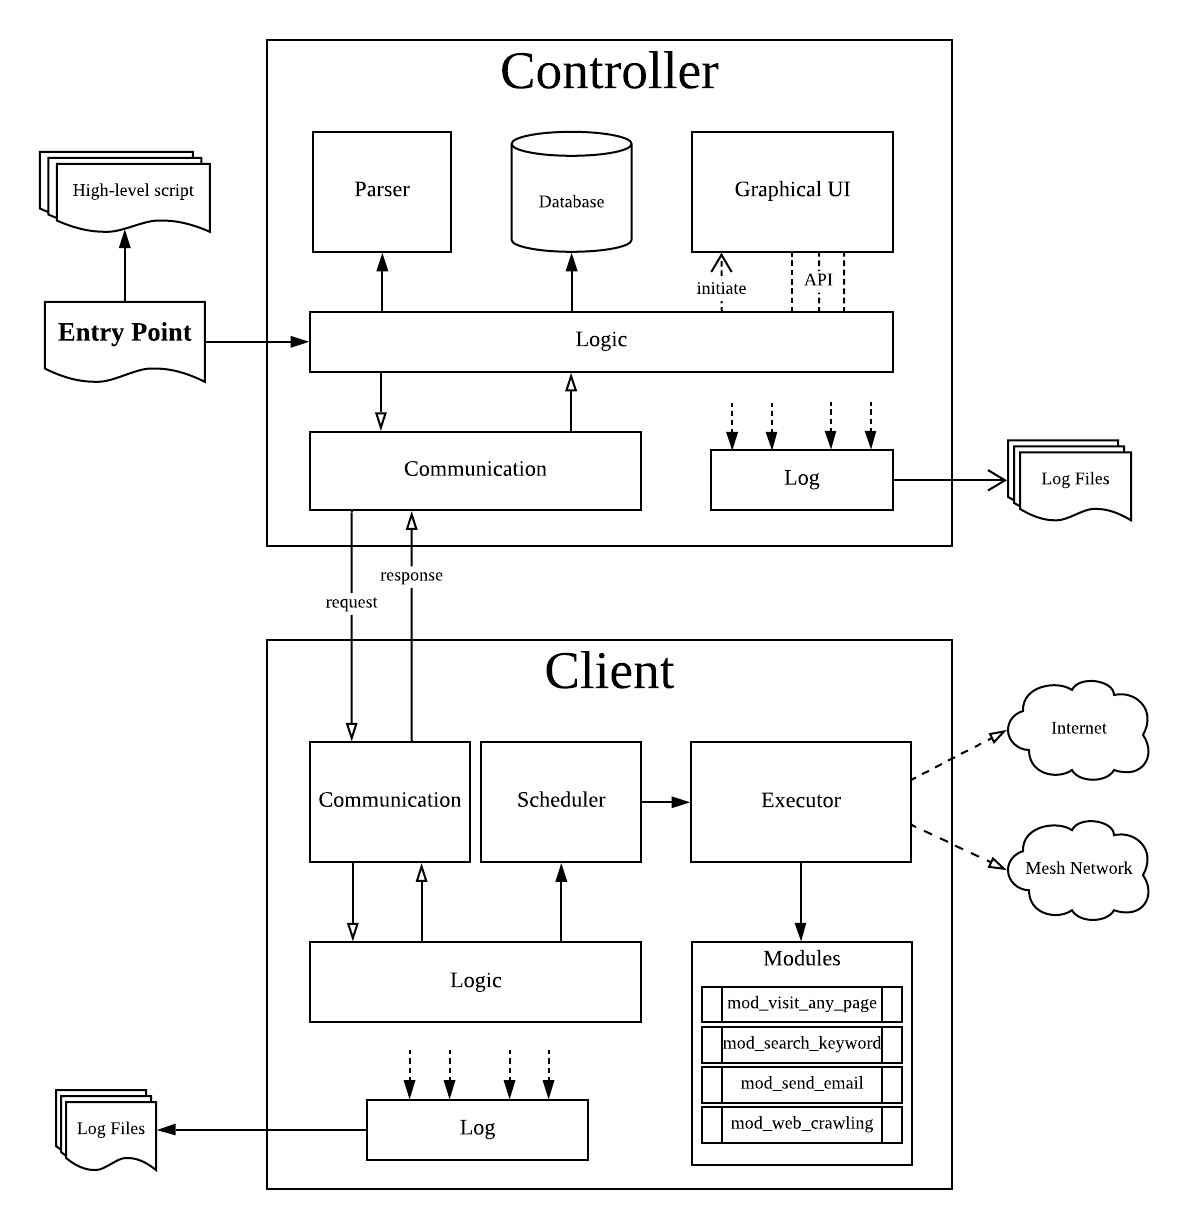
\includegraphics[width=1\textwidth]{./pictures/autraff-arc}
	\caption{Software Architecutre of Autraff}
\end{figure}


\subsection{Controller}
\subsubsection{Entry point}
Entry point is where the user uses to start up the controller-side framework. It takes all user configuration files as well as other user input files such as the the high-level script that we are going to illustrate later.

\subsubsection{Logic}
The entry point will start the logic component on controller side, and logic will start other components including parser, database, graphical ui and communication sector. After start, the logic component will also provide APIs through the graphical UI component for the user to control some of the controller or give instructions to the controllers.

\subsubsection{Parser}
The parser component is a component where all user configuration and our high-level script will be parsed into program parameters or objects, some of which will be then saved into database or displayed through graphical UI.

\subsubsection{Graphical UI}
The graphical UI will be the main interface for users to interacted with the logic controller or to instruct client nodes (inditectly through controller) after the user starts the controller program through the entry point. For example, after the controller has started, the user may want to schedule a job on a certain client, he or she may go to a specific UI page and schedule that job there.

\subsubsection{Communication Component}
The communication component will be mainly responsible for all information exchanges between the controller and each of its clients. The communication pattern will mainly be ``requests and response" format, and the controller is always pulling information and updates from all its clients, whereas there will be no way for the client to pushing information to the controller unless requested.

\subsubsection{Log Component}
This component will be mainly in charge of the logging logics of all other components. All other components except for the graphical ui will be using it for logging.

\subsection{Cient}

\subsubsection{Logic}
The logic component on the client side orchestrates all other components and manages the logic and data flow among other components. The logic component here is also a so-called entry point of the client-side program. On the client side, the user will start up the logic component first to establish the connection between this client to the controller.

\subsubsection{Communication Component}
The communication component on the client side will keep listening on the requests sent by the controller. It will pass all the request to logic compoent and the logic component will handle accordinglly. 

\subsubsection{Scheduler}
The scheduler will be instructed by the logic component and schedule the jobs accordingly on the client machine. Everytime there is a job to be executed, the scheduler will call the executor, and the executor will execute the module that defined in this job.

\subsubsection{Executor}
The executor will execute the actual jobs according to the instructions from either the scheduler component or the executor itself. If a job is scheduling based (i.e. the job is defined with a start time or an interval), then the scheduler will instruct the executor to execute this job based on its schedule. If a job is event triggered (i.e. the job does not have a start time nor an interval, but it will be executed based on the successful or failing execution of another job), then the execution of this job will be triggered after the executor executes the tiggering job. 

\subsubsection{Module}
The module here refers to a type of ``actions". For example, module ``mod\textunderscore visit\textunderscore any\textunderscore page" and module `` mod\textunderscore serach\textunderscore keyword". Each standalone module may have nothing special, but is just a single script or program. Each module may takes a few arguments, each of which will decide the actual behaviors of the module during execution. 

\section{High-Level Script}

The high-level scripts will be used as a ``user configuration" files in our framework, which will only be stored and used on the controller side. The users will use the scripts to specify and define where and how the traffic will be generated. Basically, we will needs two types of high-level scripts (written in YAML), one of which will specify all the information of clients that will be involved in generating the web traffic, while the other one will be used to specify the chain of actions to be done by different clients.

\subsection{Script of client information}

In the script defining the client node, the syntex will be rather simple and each YAML ``object" is referring to a certain client including the information about IP address (the ip address used to connect this machine from the server/controller), operating system and system version. An example of the script is shown in the figure below:\\

\begin{figure}[h!]
	\centering
	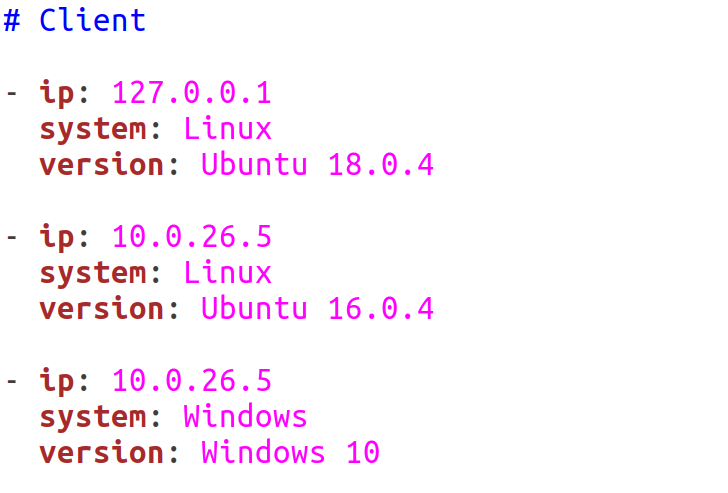
\includegraphics[width=0.6\textwidth]{./pictures/client-template}
	\caption{Example of script of client information}
\end{figure}

In the script describe above, the controller will use `ip' field to connect to and differentiate each client, and for each client, they will have and only have one unique `ip'.

\subsection{Script of job information}

During the design process of the script of job informations, we refers to the idea from Yoshka \cite{Yoshka} and Cryton \citep{Cryton}. We give users the capabilities to define binary behavior tree of actions/jobs in the script. A snapshot of a sample script is shown in the figure below.\\

\begin{figure}[h!]
	\centering
	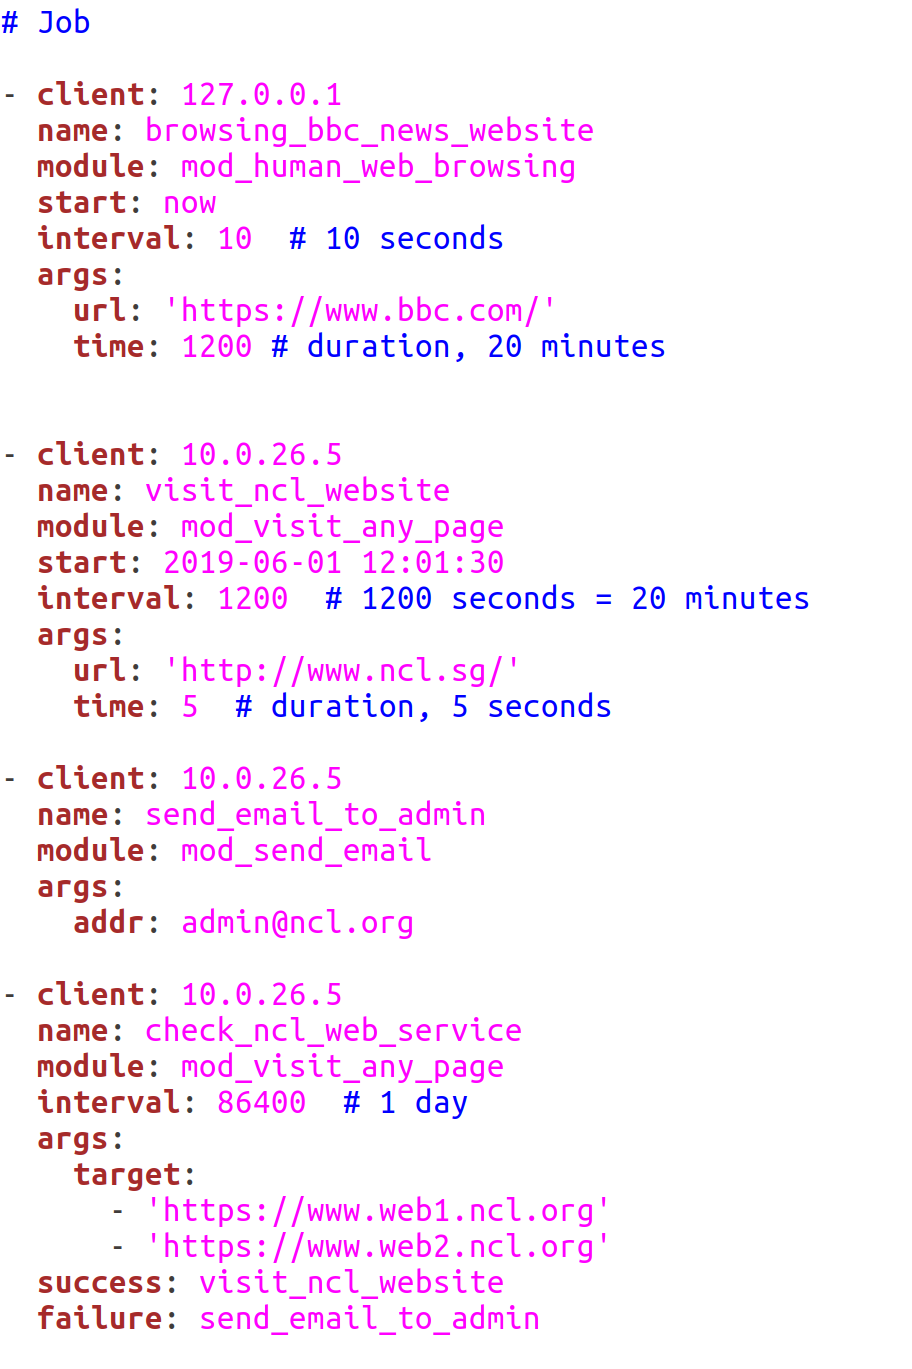
\includegraphics[width=0.6\textwidth]{./pictures/job-template}
	\caption{Example of script of job information}
\end{figure}

In the example above, each job will have compulsory attributes such as:

\begin{itemize}
\item \textbf{client} an ip address to specify on which client the job is to be executed (Note that the client ip must exist in the script of client information)
\item \textbf{name} a unique alias of the job
\item \textbf{module} the module used in this job
\end{itemize}

There are also optional attributes that will give a job more capabilities or responsibilities:

\begin{itemize}
\item \textbf{start} the start time of a job (If the start time is not specified, then it means that the job will be either triggered by other jobs or the user will schedule this job mannually. If the start time is specified as now, then right after the controller starts, the controller will tell the client to schedule the job immediately.)
\item \textbf{interval} the time interval between two consecutive execution of a job (If this is not specified, the job will be either triggered by other jobs or it will only be executed once.)
\item \textbf{args} the arguments that will be passed into the module during execution of the job (This attribute can be empty only when the module used in this job requirs no arguments.)
\item \textbf{success} the job that will be executed if this job is executed successfully
\item \textbf{failure} the job that will be executed if execution of this job fails (Both success and failure attribute will contribute to the binary behavior tree of actions.)
\end{itemize}

To illustrate more on the scenario described in the figure above: there are four jobs defined in the script -- one of them will be scheduled on client 127.0.0.1 (which is localhost, the same as the controller machine), and three of them will be executed on client 10.0.26.5. To be more specific:

\begin{enumerate}
\item job \textbf{browsing\textunderscore bbc\textunderscore news\textunderscore website}: This job will be executed on client 127.0.0.1 and it will make use of module ``mod\textunderscore human\textunderscore web\textunderscore browsing". It will be scheduled right after the controller is up with an interval of 10 seconds.

\item job \textbf{visit\textunderscore ncl\textunderscore website}: This job will be scheduled according to its start time and interval duration accordingly. Besides, this job can also be triggered by the successful execution of job ``check\textunderscore ncl\textunderscore web\textunderscore service".

\item job \textbf{send\textunderscore email\textunderscore to\textunderscore admin}: This job is defined without a start time or an interval, thus it can only be triggered when the excution of job ``check\textunderscore ncl\textunderscore web\textunderscore service" fails.

\item job \textbf{check\textunderscore ncl\textunderscore web\textunderscore service}: This job will only be scheduled when the user explicitly schedules it from the controller UI. Upon being scheduled, the job will be run once every day. For every execution, if it is successful, then job ``visit\textunderscore ncl\textunderscore website" will be executed for once, otherwise, job ``send\textunderscore email\textunderscore to\textunderscore admin" will be executed for once.
\end{enumerate}

Thus as a result, in the example above, jobs defined on client 10.0.26.5 will result in a simple binary behavior tree, which can be illustrated by the figure below:

\begin{figure}[h!]
	\centering
	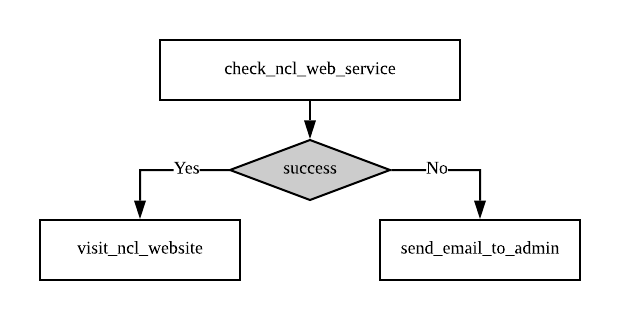
\includegraphics[width=0.6\textwidth]{./pictures/template-bbt}
	\caption{Binary behavior tree generated according to the template script of job
	\label{fig:temp-bbt} information}
\end{figure}

As more jobs are added in the high-level script, a more complex behavior tree will be generated, which may includes iterations or recursions.

\section{Implementation Details}

In this section, we will talk about the actual implementation in more details. We will firstly explain the implementation details of the communication components on both controller and client side, followed by the components details on the client side, and lastly we will address the controller side.

\subsection{Communication}

As for communication component, we are using osBrain \citep{osBrain}, a general-purpose multi-agent system module, which could be used in a distributed system for message exchanging between the server and clients.

The figure shown below roughly describes how the communication are established between the client node and the controller node. More details will be explained.

\begin{figure}[h!]
	\centering
	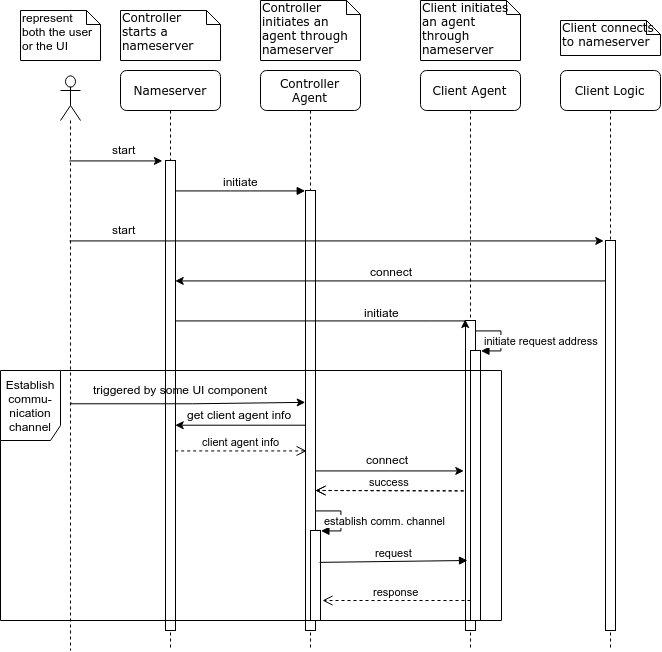
\includegraphics[width=1\textwidth]{./pictures/comm-uml}
	\caption{Binary behavior tree generated according to the template script of job information}
\end{figure}

Every time the user starts up the controller side framework, a nameserver will be running on the controller machine and a agent will also be initiated to represent the controller node. Before all the jobs are scheduled, the user needs to go to each client machine and start up the client side program (basically the logic component as described in previous section). The client will firstly try to connect to the nameserver and then initiated another agent to represent itself.\\

After initiation, the client agent will initiate a special ``address" (a special object in osBrain terminolog) for recieving request and dispatching response. Then the user on the controller side will decide or trigger an event to make the controller agent connect to the client agent. The controller agent will firstly get the client agent information from the nameserver and then it will try to established a tcp connection with the client agent. If it succeeds, then the controller agent will initiated a ``connection" object (another special object in osBrain terminolog) which will be used directly for future request and response communication.


\subsection{Client}
\subsubsection{Logic}
The logic component on client side is implemented as a wrapper python script of all other components. It is in charge of the establishment of the client agent and the communication ``address", as well as to instruct the scheduler component to schedule certain jobs when such requests are recieved from the communication channel.

\subsubsection{Module \& Executor}
Each module in Autraff is implemented as a standalone python script where there will be only one function called ``execute" is defined. And the concept of executor defined in previous section will only be an abstract concept, and there will be no concrete and explicit implementaion of the executor. The skeleton of the function is define as following:

\begin{lstlisting}
def execute(args, driver=None):
    # function body
    return driver
\end{lstlisting}

``arg" is a dictionary object that contains all compulsory and optional arguments needed for executing a certain module. ``driver" is a Selenium web driver object which will be used to perform the real web browsing actions. If the execution of the module is triggered by a predecessor module, then the predecessor will pass the driver used by itself to its successor module, otherwise, a new driver will be initiated by the module itself.\\

For the declaration of a module\textquotesingle s successors (i.e. the success and failure field specified in the high level script), they will be passed together inside the ``args" dictionary. For the binary behavior tree descirbe in figure \ref{fig:temp-bbt}, the args parameter in module ``mod\textunderscore visit\textunderscore any\textunderscore page" used by job ``check\textunderscore ncl\textunderscore web\textunderscore service" will be constructed as:

\begin{lstlisting}
args = {
    target: ['https://www.web1.ncl.org',
             'https://www.web2.ncl.org'],
    success: {
        module: 'mod_visit_any_page',
        args: {
            url: 'https://www.ncl.sg/',
            time: 5,
        },
    },
    failure: {
        module: 'mod_send_email',
        args: {
            addr: 'admin@ncl.org'
        }
    },
}
\end{lstlisting}

And as for the return value, a module will always return the driver object that it uses. If this module is called by the scheduler, then the return value will have no meaning, but it will make sense to a module\textquotesingle s predecessors if this module is trigger or used by other module. \\

Here we will list some most useful modules that have already been implemented:
\begin{itemize}
\item \textbf{mod\textunderscore visit\textunderscore any\textunderscore page}: this module will take a url as a compulsory argument and visit and stay on this web page for a certain amount of time.
\item \textbf{mod\textunderscore search\textunderscore key\textunderscore word}: this module will take a keyword as a compulsory argument and search this keyword using a popular searching engine as specified in another argument. And then finally click on one of the searching result.
\item \textbf{mod\textunderscore human\textunderscore web\textunderscore browsing}: this module will take a url as a compulsory argument and start to crawl from this web page, which will give a simulation of how a real human is browsing the web. The underlining theory and algorithms used will be explained in the following chapter.
\item \textbf{mod\textunderscore send\textunderscore email}: this module will take an email address as a compulsory argument and send an email to this address. The user can also specify the username and password to be used to send the email, as well as the email subject and body.
\end{itemize}


\subsubsection{Scheduler}
As for the scheuler implementation on the client side, we made use of the APScheduler (Advanced Python Scheduler) library \citep{APScheduler}, which could help to schedule to execute python code either periodically or at a fixed time.\\

Each client node will have exectly one background sheduler defined in logic component, and it will be initiated as long as the user starts the client side program. The figure below roughly illustrates how the scheduler works in our context.\\

\begin{figure}[h!]
	\centering
	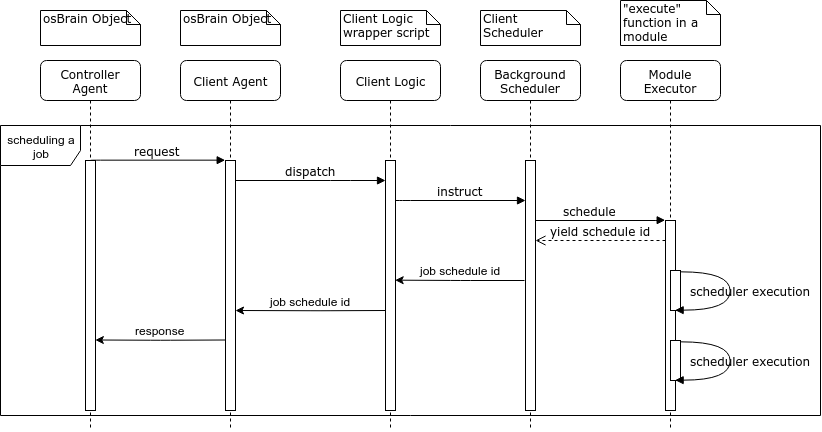
\includegraphics[width=1\textwidth]{./pictures/scheduler-uml}
	\caption{Sequence diagram of how scheduler works.}
\end{figure}

To illustrate, every time there is a request regarding scheduling or stopping a job sent from the controller to the client, the client logic will resolve the request body and then give the instructions to background scheduler. And if nothing goes wrong, the logic component will response the controller with success message.\\

In such manner, both the controller and the client logic component will not be aware of what is happeing to the actual execution of a job if not requested. But the log component will always keep track on all the subtle changes happening in this system.


\subsubsection{Log}
The log component on the client side mainly consist of two part. One is a general logger object, which can be access anywhere in any components. By using this logger, each component can specify where to write their logging messages or just to a global general log file. Another one comes as a python decorator, which will be used when defining or developing each of the modules. Afther being wrapped by this logger decorator, the logging system will output with a standard format to record the modules and jobs execution. And now, a sample module will be defined as:

\begin{lstlisting}
@log_mod_execution
def execute(args, driver=None):
    # function body
    return driver
\end{lstlisting}

\subsection{Controller}
\subsubsection{Parser \& Database}
The implementation of parser is done by yaml reader in python standard library. It will take the input file (i.e. the high level script) and the parse them into python object which the logic component could understand.\\

After parsing, the logic component will store all the parsed information into the relational database which is implemented using SQLite database. The database mainly consists of two tables, one of which stores the information about clients, and the other one stores the information about the jobs. The figure below shows the schema of the relational database.

\begin{figure}[h!]
	\centering
	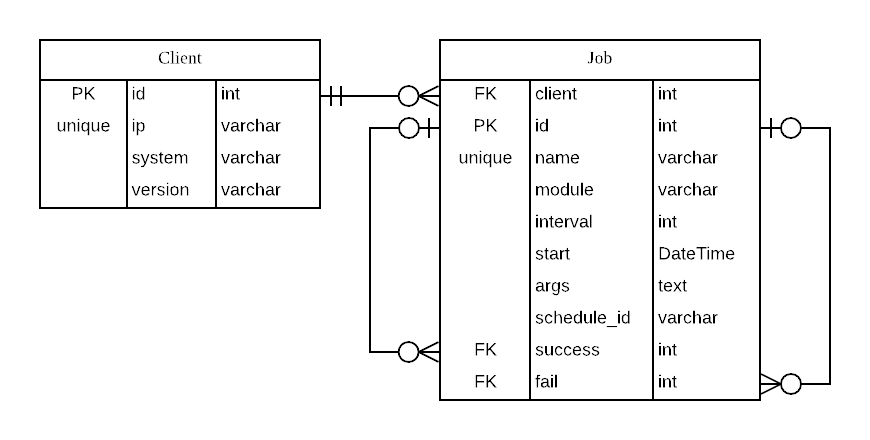
\includegraphics[width=1\textwidth]{./pictures/db-schema}
	\caption{Controlle database schema diagram.}
\end{figure}



\subsubsection{Logic \& Backend}

\subsubsection{UI \& Frontend}


\subsection{Use Case by Sequence Diagram}


\section{Limitations about Current Implementation}
1. after starting the server, we have to manually start the client before scheduling



\chapter{Literature Review: Human Web Browsing Simulation} \label{lr:hwbs}

\chapter{Mathmatical Modeling: Human Web Browsing Simulation} \label{mm}

\chapter{Testing and Validation} \label{tv}

\chapter{Conclusions}
\section{Smmary}
\section{Limitation}
\section{Future work}



\bibliography{reference}
\bibliographystyle{apalike}

\end{document}

